%\documentclass{article}
\documentclass[12pt,a4paper]{article}
\usepackage[utf8]{vietnam}

%\usepackage{url}
%\usepackage{hyperref}

%\usepackage{flafter}
\usepackage[T1,hyphens]{url}
\usepackage{enumitem}
\usepackage{natbib}
\usepackage{cancel}
 \usepackage{xspace}
\usepackage{graphicx}
\usepackage{multicol}
\usepackage{multirow}
\usepackage{subfig}
\usepackage{amsmath}
\usepackage{amssymb}
\usepackage[a4paper, width=186mm, top=18mm, bottom=18mm, includeheadfoot]{geometry}
%\usepackage[a4paper, width=140mm, top=18mm, bottom=22mm, includeheadfoot]{geometry}
\usepackage{booktabs}
\usepackage{array}
\usepackage{verbatim}
\usepackage{caption}
\usepackage{natbib}
\usepackage{booktabs}
\usepackage{float}
\usepackage{pdflscape}
\usepackage{mathtools}
\usepackage[usenames, dvipsnames]{xcolor}
\usepackage{afterpage}
\usepackage{pgf}
\usepackage{tikz}
\usepackage{adjustbox}
%\usepackage{pgfplots}
%\pgfplotsset{compat=newest}
%\usepackage{dirtree}
\usepackage[style=american]{csquotes}
\usepackage{amsfonts}
\usepackage{tikz}
\usepackage{tkz-graph}
\usetikzlibrary{arrows,decorations.pathmorphing,automata,positioning,backgrounds,fit,shapes.symbols,chains,intersections}

\newtheorem{definition}{Định nghĩa}[section]
\newtheorem{theorem}{Theorem}[section]
\newtheorem{lemma}{Lemma}
\newtheorem{proof}{Proof} [section]

\usepackage[toc, page, title, titletoc, header]{appendix}
\usepackage{marginnote}
\usepackage{tablefootnote}

\renewcommand\appendixname{Phụ lục}
\renewcommand\appendixpagename{Phụ lục}
\renewcommand\appendixtocname{Phụ lục}
\renewcommand\abstractname{Abstract}


\usepackage{perpage} %the perpage package
\MakePerPage{footnote} %the perpage package command

\usetikzlibrary{shapes.geometric}%
\usepackage{color}
%\usepackage[pages=some, placement=top]{background}
\usepackage{eso-pic}
\usepackage[final]{pdfpages}

%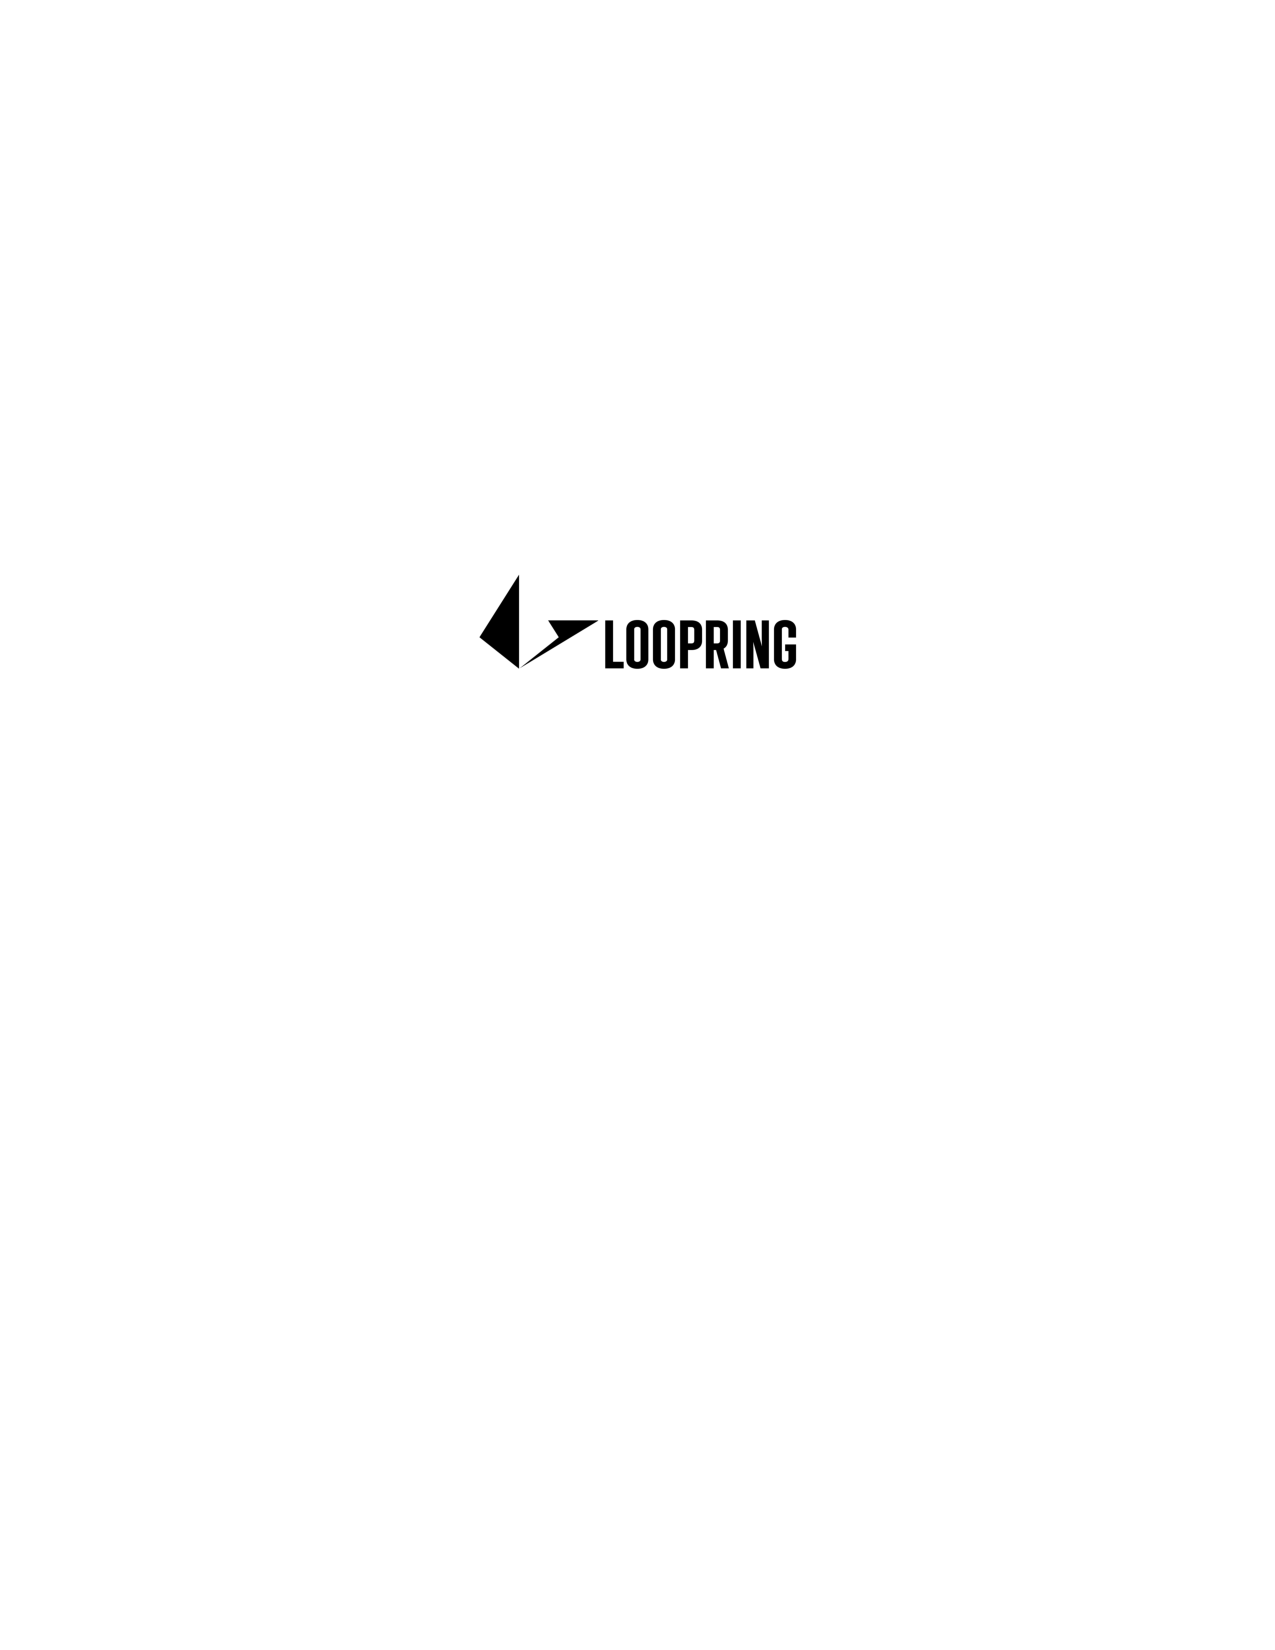
\includepdf[pages=1]{cover}
\hyphenpenalty=750

\title{\textbf{Loopring:}\\\textbf{Giao thức trao đổi Token phân tán}}
\author{
  Daniel Wang\\
  \texttt{daniel@loopring.org}\\
  \and
  	Jay Zhou\\
  	\texttt{jay@loopring.org}\\
  	\and
  	Alex Wang\\
  	\texttt{alex@loopring.org}\\
  	\and
  	Matthew Finestone\\
  	\texttt{matt.finestone@gmail.com}\\
  \\
  \texttt{https://loopring.org}
 }

\makeatletter
\def\CTEX@section@format{\Large\bfseries}
\makeatother

\makeatletter
\newenvironment{tablehere}
 {\def\@captype{table}}
 {}

\newenvironment{figurehere}
 {\def\@captype{figure}}
 {}
\makeatother
%
%\newcommand\BackgroundPic{%
%\put(0, 0){%
%\parbox[b][\paperheight]{\paperwidth}{%
%\vfill
%\centering
%\includegraphics[width=\paperwidth, height=\paperheight, %
%%keepaspectratio]{images/background.jpg}%
%]{images/background.jpg}%
%\vfill
%}}}


\begin{document}
\maketitle

\begin{abstract}
Loopring là một giao thức mở cho việc xây dựng các giao dịch phi tập trung.  Loopring hoạt động như một tập hợp công khai của các hợp đồng thông minh có trách nhiệm trao đổi và thanh toán, cùng với một nhóm off-chain tổng hợp và truyền đạt các trao đổi. Giao thức này là miễn phí, có khả năng mở rộng và phục vụ như một khối xây dựng được chuẩn hóa cho các ứng dụng phân cấp (dApps) kết hợp chức năng trao đổi. Các tiêu chuẩn tương thích của nó giúp trao đổi thuận tiện cho giao dịch ẩn danh và không cần đặt niềm tin vào bất kỳ ai. Một cải tiến quan trọng đối với các giao thức trao đổi phân quyền hiện nay là khả năng làm cho các lệnh có thể trộn lẫn và trùng khớp với các lệnh khác, các lệnh không giống nhau, loại bỏ các ràng buộc của các cặp giao dịch hai token và cải thiện đáng kể khả năng thanh khoản. Loopring cũng sử dụng một giải pháp độc đáo và mạnh mẽ để ngăn chặn lỗi front-running: là một nỗ lực không công bằng để gửi các giao dịch thành một khối nhanh hơn nhà cung cấp giải pháp ban đầu. Loopring là một chuỗi khối bất khả tri, và có thể triển khai trên bất kỳ chuỗi khối nào với chức năng hợp đồng thông minh. Vào thời điểm viết, nó hoạt động trên Ethereum [1] [2] và Qtum [3] với NEO [4] đang được xây dựng.
\end{abstract}

\begin{multicols}{2}
\section{Giới thiệu\label{sec:introduction}}
Với sự gia tăng của các loại hình tài sản trên chuỗi khối blockchain, nhu cầu trao đổi tài sản giữa những cá thể hay tổ chức đã tăng lên đáng kể. Khi hàng ngàn tiền mã hóa mới được giới thiệu - bao gồm cả việc mã hóa các tài sản truyền thống - nhu cầu này được mở rộng. Cho dù trao đổi các loại tiền mã hóa để thúc đẩy đầu cơ thương mại, hay chuyển đổi để truy cập mạng thông qua các các loại tiền mã hóa tiện ích bản địa, khả năng trao đổi một tài sản mã hóa cho khác là nền tảng cho các hệ sinh thái lớn hơn. Thật vậy, có một sức mạnh tiềm năng trong tài sản [5], và nhận thức sức mạnh này - mở vốn - đòi hỏi không chỉ xác nhận quyền sở hữu mà blockchains đã được phép cho phép, mà còn là khả năng tự do chuyển đổi và biến đổi các tài sản này.
Như vậy, trao đổi tiền mật mã mà không cần đặt niềm tin vào bất kỳ ai là một điểm khai phá cho công nghệ blockchain. Cho đến bây giờ, những người đam mê Crypto đã giải quyết phần lớn việc giao dịch tiền mã hóa trên các sàn giao dịch tập trung truyền thống. Cần phải có giao thức Loopring bởi vì cũng giống như Bitcoin [6] đã nhấn mạnh một cách nghiêm túc rằng, đối với tiền điện tử peer-to-peer, "những lợi ích chính sẽ mất nếu một bên thứ ba đáng tin cậy vẫn phải ngăn ngừa việc chi tiêu gấp đôi" cũng là những lợi ích chính của tài sản phi tập trung bị mất nếu họ phải vượt qua các sàn giao dịch tập trung.
Giao dịch các loại tiền mã hóa phân quyền trên các sàn giao dịch tập trung không có ý nghĩa từ quan điểm triết học, vì nó không giữ được các phẩm chất mà các dự án phi tập trung này tán thành. Có nhiều rủi ro thực tế và hạn chế trong việc sử dụng các sàn giao dịch tập trung được mô tả dưới đây. Các sàn giao dịch phi tập trung (DEXs) [7] [8] [9] đã tìm cách giải quyết những vấn đề này, và nhiều trường hợp đã thành công trong việc làm giảm các nguy cơ bảo mật bằng việc sử dụng các chuỗi khối để cắt giảm trung gian. Tuy nhiên, khi DEX trở thành cơ sở hạ tầng quan trọng cho nền kinh tế mới, sẽ có nhiều cải thiện hiệu suất. Loopring nhắm tới mục tiêu cung cấp các công cụ mô đun cho cơ sở hạ tầng nói với giao thức mở không đồng thuận dApp của nó.

\section{Tổng quan giao dịch hiện nay\label{sec:current_exchange_landscape}}

\subsection{Các bất cập của các sàn giao dịch tập trung}
Ba rủi ro chính của các cuộc sàn giao dịch tập trung là; 1) Thiếu bảo mật, 2) Thiếu sự minh bạch, và 3) Thiếu thanh khoản.
Thiếu an toàn phát sinh từ việc người dùng thường từ bỏ sự kiểm soát các mã khóa của họ (quỹ) cho một thực thể tập trung. Điều này dẫn tới người dùng có thể bị mất tài sản nếu sàn tập trung đó bị hack. Các rủi ro về an ninh và hack phải đối mặt với tất cả các sàn giao dịch tập trung được biết đến [10] [11], nhưng thường được chấp nhận như là "bảng stakes" cho việc giao dịch tiền mã hóa. Các sàn giao dịch tập trung tiếp tục trở thành cơ chế honeypots cho các hacker tấn công vì các máy chủ của họ có quyền giám sát hàng triệu đô la của các quỹ người dùng. Các nhà phát triển giao dịch cũng có thể đưa ra các lỗi sai số không trung thực, vô tình với các khoản tiền của người sử dụng. Đơn giản là người dùng không kiểm soát các thẻ mã hoá của riêng mình khi gửi vào một sàn giao dịch tập trung.
Thiếu Minh bạch sẽ làm cho người dùng gặp nguy cơ giao dịch không trung thực diễn ra một cách không công bằng. Sự khác biệt ở đây là do thiếu minh bạch của các nhà điều hành sàn giao dịch vì người dùng không thực sự buôn bán tài sản của họ trên các sàn giao dịch tập trung, mà là một IOU. Khi các Token được gửi đến ví của sàn, sàn đó sẽ tạm giữ và cung cấp một IOU ở vị trí của nó. Tất cả các giao dịch sau đó sẽ diễn ra giữa các IOU của người dùng. Để rút tiền, người dùng sẽ sử dụng IOU của họ với sàn giao dịch, và nhận Token của họ vào địa chỉ ví ngoại lệ của họ. Trong suốt quá trình này, có thể thiếu sự minh bạch và việc trao đổi có thể hủy, đóng băng tài khoản, phá sản ...; Họ có thể sử dụng tài sản của người dùng cho các mục đích khác trong thời gian lưu ký, như cho vay đối với bên thứ ba. Sự thiếu minh bạch có thể làm tăng chi phí cho người sử dụng, chẳng hạn như chi phí giao dịch cao hơn, sự chậm trễ khi có nhu cầu cao điểm, rủi ro về luật lệ và các lệnh đang chạy phía trước.
Thiếu thanh khoản. Từ quan điểm của các nhà quản lý sàn giao dịch, tính thanh khoản bị phân mảnh cản trở việc lối vào bằng các sàn giao dịch mới vì hai kịch bản thắng-lấy-tất cả. Thứ nhất, giao dịch với số lượng lớn nhất của cặp giao dịch chiến thắng, bởi vì người dùng nhận thấy nó mong muốn để thực hiện tất cả các giao dịch của họ trên một sàn giao dịch. Thứ hai, việc trao đổi với bảng đấu giá Order Book lớn nhất sẽ thắng, bởi vì hoạt động trả giá-đặt giá mở rộng cho mỗi cặp giao dịch. Điều này không khuyến khích sự cạnh tranh từ những người mới đến bởi vì họ rất khó khăn trong việc xây dựng thanh khoản ban đầu. Kết quả là nhiều cuộc giao dịch đòi hỏi thị phần cao mặc dù có sự phàn nàn của người dùng và thậm chí các sự cố về hacker. Cần lưu ý rằng khi các sàn tập trung giành chiến thắng về thị phần, chúng trở thành một mục tiêu hacking lớn hơn bao giờ hết.
Từ quan điểm của người dùng, tính thanh khoản bị phân mảnh làm giảm đáng kể trải nghiệm người dùng. Trong một sàn giao dịch tập trung, người dùng chỉ có thể giao dịch trong phạm vi tài sản thanh khoản của chính sàn đó, chống lại với bảng đấu giá của mình và giữa các cặp Token được hỗ trợ. Để trao đổi Token A cho token B, người dùng phải đi đến một sàn giao dịch hỗ trợ cả hai Token hoặc đăng ký tại cácsàn giao dịch khác nhau, dẫn tới tiết lộ thông tin cá nhân. Người dùng thường phải thực hiện các giao dịch sơ bộ hoặc trung gian, thường là sử dụng BTC hoặc ETH, dẫn tới mất phí trả giá hay đặt giá mong muốn bán. Cuối cùng, các bảng đấu giá có thể không đủ sâu để hoàn thành giao dịch mà không có sự trượt giá hữu hình. Ngay cả khi sàn giao dịch có mục đích xử lý khối lượng lớn, không có đảm bảo rằng khối lượng và thanh khoản không phải là giả mạo [12].
Kết quả là tình trạng thanh khoản bị ngắt kết nối và một hệ sinh thái bị phân mảnh tương tự như hệ thống tài chính kế thừa, với khối lượng giao dịch đáng kể được tập trung ở một vài giao dịch. Các cam kết thanh khoản toàn cầu của các chuỗi khối không có giá trị trong các trao đổi tập trung.
\subsection{Các bất cập của các sàn giao dịch phi tập trung}
Các sàn giao dịch phi tập trung khác với các sàn giao dịch tập trung một phần bởi vì người dùng duy trì quyền kiểm soát các mã khóa cá nhân Prive-key (tài sản) bằng cách thực hiện giao dịch trực tiếp trên nền tảng blockchain. Bằng cách tận dụng công nghệ Trustless (không cần đặt tin tưởng vào bất kỳ ai) của chính mình, họ thành công trong việc giảm thiểu nhiều rủi ro về bảo mật. Tuy nhiên, vẫn tồn tại vấn đề liên quan đến hiệu suất và những hạn chế cơ cấu.
Tính thanh khoản thường là một vấn đề vì người dùng phải tìm kiếm các đối tác thông qua các nguồn và tiêu chuẩn thanh khoản khác nhau. Các hiệu ứng thanh khoản bị phân mảnh hiện diện nếu DEXs hoặc dApps nói chung không sử dụng các tiêu chuẩn nhất quán để tương tác, và nếu các lệnh không được chia sẻ / tuyên truyền qua một mạng lưới rộng. Tính thanh khoản của các sổ cái giới hạn, và cụ thể là khả năng phục hồi của chúng - các lệnh giới hạn đã được làm mới nhanh chóng - có thể ảnh hưởng lớn đến các chiến lược kinh doanh tối ưu [13]. Sự vắng mặt của các tiêu chuẩn như vậy đã không chỉ dẫn đến việc giảm thanh khoản, mà còn liên quan đến một loạt hợp đồng thông minh độc quyền không an toàn.
Hơn nữa, kể từ khi các giao dịch được thực hiện trên chuỗi, DEX thừa kế các hạn chế của nền tảng blockchain, cụ thể là: khả năng mở rộng, sự chậm trễ trong thực hiện (khai thác mỏ), và các sửa đổi tốn kém cho các lệnh. Do đó, bảng đấu giá chuỗi khối không tỷ lệ tốt, vì thực hiện mã trên chuỗi khối phải chịu một chi phí (gas), làm cho việc hủy các lệnh dẫn tới nhiều tốn kém.
Cuối cùng, bởi vì các lệnh mua bán là công khai, việc giao dịch để đặt một lệnh mua bán có thể được nhìn thấy bởi các thợ mỏ vì nó đang chờ được khai thác vào khối kế tiếp và được đặt vào một bảng đấu giá. Sự chậm trễ này làm cho người sử dụng gặp nguy cơ chạy trước và các bước thực thi hay giá chống lại anh ta.
\subsection{Giải pháp Lai}
Vì những lý do trên, các sàn giao dịch thuần túy dựa trên blockchain có những hạn chế làm cho chúng không cạnh tranh với các sàn tập trung. Có một sự cân bằng giữa sự on-chain thuộc về tính không cần đặt tin tưởng vào ai, và tốc độ trao đổi tập trung và sự linh hoạt của lệnh. Các giao thức như Loopring và 0x [14] mở rộng một giải pháp giải quyết on-chain với quản lý các lệnh bằng off-chain: giải pháp mở rộng không trực tiếp trên blockchain. Các giải pháp này xoay quanh các hợp đồng thông minh mở, nhưng điều chỉnh các hạn chế về khả năng mở rộng bằng cách thực hiện một số chức năng off-chain và cho phép các nút linh hoạt trong việc thực hiện các vai trò quan trọng cho mạng. Tuy nhiên, vẫn còn những hạn chế đối với mô hình lai [15]. Giao thức Loopring đề xuất những khác biệt có ý nghĩa trong cách tiếp cận của chúng ta đối với một giải pháp lai trong trang này.

\section{Giao thức Loopring \label{sec:loopring_protocol}}
Loopring không phải là một sàn giao dịch phân tán, nhưng là một giao thức mô đun để xây dựng các sàn giao dịch phân tán trên nhiều nền tảng blockchains. Chúng tôi tháo rời các bộ phận cấu thành của một sàn giao dịch truyền thống và đưa ra một bộ hợp đồng thông minh công khai và các bên phân quyền ở vị trí của nó. Các vai trò trong mạng bao gồm ví, rơle, chuỗi khối hiệp hội chia sẻ thanh khoản, các trình duyệt bảng đấu giá, Vòng Thợ đào Ring-Miners, và các dịch vụ mã hóa tài sản. Trước khi xác định mỗi vai trò, trước tiên cần hiểu các lệnh Loopring.

\subsection{Vòng lệnh\label{sec:order_ring}}
Các lệnh của Loopring được thể hiện trong những gì chúng tôi gọi là Mô hình lệnh một hướng (UDOM) [16]. UDOM thể hiện các lệnh như các yêu cầu trao đổi Token, số lượng S / số lượng B, (sô lượng để bán / mua) thay vì đặt giá và đấu giá. Vì mỗi lệnh mua bán chỉ là một tỷ giá hối đoái giữa hai token, một tính năng mạnh mẽ của giao thức là việc trộn và kết hợp nhiều lệnh mua bán trong giao dịch tròn. Bằng cách sử dụng tối đa 16 lệnh thay vì một cặp giao dịch đơn, sẽ có sự gia tăng về tính thanh khoản và sự cải thiện về giá.

\begin{center}
\begin{figurehere}
\centering
\tikzstyle{block} = [draw, fill=blue!20, rectangle,
    minimum height=3em, minimum width=6em]
\tikzstyle{sum} = [draw, fill=blue!20, circle, node distance=1cm]
\tikzstyle{input} = [coordinate]
\tikzstyle{output} = [coordinate]
\tikzstyle{pinstyle} = [pin edge={to-,thin,black}]

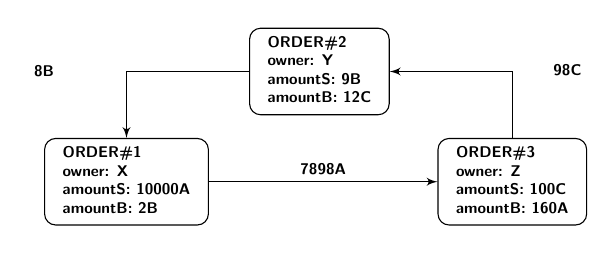
\begin{tikzpicture}[
    auto,
    node distance=2cm,
    >=latex',
    font=\bfseries\footnotesize\sffamily,
    order/.style={
		scale=0.7,
		rectangle,
		rounded corners,
		draw=black,
		text centered,
%		text width=5cm,
		minimum height=12mm,
		fill=white
	},
	label/.style={
		scale=0.7
	}
  ]
    % We start by placing the blocks

  \node [order] (order2)
 {%
 \begin{tabular}{l}
  \textbf{ORDER\#2}\\
  \textbf{owner: Y}\\
  \textbf{amountS: 9B}\\
  \textbf{amountB: 12C}
 \end{tabular}
 };

  \node [order, below of=order2, xshift=-3.5cm] (order1)
 {%
 \begin{tabular}{l}
  \textbf{ORDER\#1}\\
  \textbf{owner: X}\\
  \textbf{amountS: 10000A}\\
  \textbf{amountB: 2B}
 \end{tabular}
 };


  \node [order, below of=order2, xshift=3.5cm] (order3)
 {%
 \begin{tabular}{l}
  \textbf{ORDER\#3}\\
  \textbf{owner: Z}\\
  \textbf{amountS: 100C}\\
  \textbf{amountB: 160A}
 \end{tabular}
 };

 \draw [draw,->] (order1) -- node [label] {\textbf{7898A}} (order3);
 \draw [draw,->] (order2) -| node [label, xshift=-1.8cm] {\textbf{8B}} (order1);
 \draw [draw,->] (order3) |- node [label, xshift=1cm, yshift=0.24cm] {\textbf{98C}} (order2);

\end{tikzpicture}

\caption{Một Vòng lệnh của 3 lệnh}
\label{fig:ring}
\end{figurehere}
\end{center}
Hình trên cho thấy một vòng lệnh gồm 3 lệnh mua bán. Mỗi token của lệnh bán (tokenS) là token của lệnh khác để mua (tokenB). Nó tạo ra một vòng lặp cho phép mỗi thứ tự để trao đổi các token mong muốn của họ mà không cần một lệnh đối lập cho cặp của nó. Các giao dịch cặp lệnh truyền thống có thể thực hiện được, chủ yếu là một trường hợp đặc biệt của một vòng lệnh.

\begin{definition}[vòng lệnh] để $C_{0}$, $C_{1}$, $\cdots$, $C_{n-1}$ thành  $n$  token khác nhau,   $O_{0\rightarrow 1}$, $\cdots$, $O_{i\rightarrow i\oplus 1}$, $\cdots$, $O_{n-1 \rightarrow 0}$ thành $n$ lệnh.  Các lệnh đó có thể biểu diễn một vòng lệnh cho giao dịch.
$$O_{0\rightarrow 1} \rightarrow \cdots \rightarrow O_{i\rightarrow i\oplus 1} \rightarrow \cdots \rightarrow O_{n-1\rightarrow 0} \text{, }$$
với $n$ là độ dài của vòng lệnh, và $i\oplus 1 \equiv i+1 \mod n$.
\end{definition}

Một vòng lệnh có giá trị khi tất cả các giao dịch thành phần có thể được thực hiện với tỷ giá hối đoái bằng hoặc tốt hơn so với tỷ lệ ban đầu được ngầm định bởi người sử dụng. Để xác minh tính hiệu lực của vòng lệnh, các hợp đồng thông minh với giao thức Loopring phải nhận được các vòng lệnh từ người khai thác vòng, nơi sản phẩm của tỷ giá hối đoái ban đầu của tất cả các lệnh bằng hoặc lớn hơn 1.

Giả sử Alice và Bob muốn trao đổi token  A và B. Alice có 15 token  A và cô ấy muốn 4 token B ; Bob có 10 mã B và anh ta muốn 30 token A.
Ai đang mua và ai đang bán? Điều này chỉ phụ thuộc vào tài sản mà chúng tôi sửa chữa để báo giá. Nếu token A là tham chiếu, thì Alice mua token B với giá ${15 \over 4} = 3.75$A, trong khi Bob bán 10 token B với giá ${30 \over 10} = 3.00$A. Trong trường hợp lấy token B làm tham chiếu, chúng tôi nói rằng Alice đang bán 15 token A với giá ${4\over 15}=0.26666667$B và Bob mua 10 token A với giá ${10 \over 30}=0.33333334$B. Do đó, ai là người mua hoặc người bán là tùy ý.

Trong trường hợp đầu Alice sẵn sàng mua với giá cao hơn (3.75A) hơn mà giá Bob đang bán token của anh ta (3.00A), trong trường hợp thứ hai Bob sẵn sàng mua với giá (0.33333334B) cao hơn mà giá Alice đang bán (0.26666667B).  Rõ ràng rằng cuộc giao dịch có thể diễn ra bất cứ khi nào người mua sẵn sàng mua với giá cao hơn hoặc bằng với giá của người bán đang bán.
\begin{equation}
{{15\over 4} \over {30\over 10}} = {{10\over 30} \over {4\over 15}}={15 \over 4} \cdot {10 \over 30} = 1.25 > 1
\end{equation}
Do đó, để có thể được lấp đầy một bộ n lệnh, toàn bộ hoặc một phần, chúng ta cần phải biết liệu sản phẩm của từng tỷ giá hối đoái như là lệnh mua có dẫn đến một số lớn hơn hay bằng 1. Nếu có, tất cả n các lệnh có thể là một phần, hoặc hoàn toàn được lấp đầy [17].
Nếu chúng tôi giới thiệu một bên thứ ba, Charlie, như vậy Alice muốn bán cho $x_1$ token A và nhận được $y_1$ token B, Bob muốn bán $x_2$ token B và nhận $y_2$ token C, và Charlie muốn bán $x_3$ token C và nhận $y_3$ token A. Các token cần thiết đã có, giao dịch có thể xảy ra nếu:

\begin{equation}
{{x_1 \cdot x_2 \cdot x_3 \over y_1 \cdot y_2 \cdot y_3} \geq 1}
\end{equation}
Xem phần 7.1 để biết thêm chi tiết về các lệnh của Loopring.

\section{Các thành phần hệ sinh thái\label{sec:ecosystem}}
Những thành phần hệ sinh thái sau đây cùng nhau cung cấp tất cả các chức năng mà một cuộc trao đổi tập trung sẽ cung cấp.
\begin{itemize}

\item \textbf{Ví:}Một dịch vụ ví thông thường hay giao diện cho phép người dùng truy cập vào token của họ và cách gửi các lệnh tới mạng Loopring. Ví tiền sẽ được khuyến khích tạo lệnh bằng cách chia sẻ lệ phí với những người khai tác vòng (xem phần 8). Với niềm tin rằng tương lai của giao dịch sẽ diễn ra trong sự an toàn của ví cá nhân của người dùng, kết nối các khoản thanh khoản này thông qua giao thức của chúng tôi là việc quan trọng nhất.

\item \textbf{Hiệp hội Chia sẻ thanh khoản Blockchain / Relay-Mesh: } Một mạng lưới Relay-mesh cho việc chia sẻ thanh khoản và lệnh. Khi các nốt chạy phần mềm chuyển tiếp Loopring, họ có thể tham gia vào một mạng hiện có và chia sẻ thanh khoản với các chuyển tiếp khác qua một blockchain của hiệp hội. Blockchain của hiệp hội mà chúng tôi đang xây dựng như là một sự thực hiện đầu tiên với việc chia sẻ lệnh thời gian thực (1-2 giây khối), và giảm bớt lịch sử cũ để cho phép tải nhanh hơn bởi các nốt mới. Đáng chú ý, các chuyển tiếp không cần phải tham gia vào hiệp hội này; họ có thể hành động một mình và không chia sẻ thanh khoản với người khác, hoặc họ có thể bắt đầu và quản lý mạng lưới chia sẻ thanh khoản của chính họ.

\item \textbf{Chuyển tiếp / các thợ khai thác vòng:}các chuyển tiếp là các nút nhận các lệnh từ ví hoặc mạng relay- mesh, duy trì các bảng đấu giá và lịch sử giao dịch, và tùy chọn phát các đơn lệnh cho các Chuyển tiếp khác (thông qua bất kỳ off-chain nào) và / hoặc các nút mạng relay-mesh. Khai thác mỏ là một tính năng - không phải là yêu cầu - của các chuyển tiếp. Đó là việc tính toán nặng và được thực hiện hoàn toàn bằng phương thức off-chain. Chúng tôi gọi các chuyển tiếp với tính năng khai thác vòng được kích hoạt bởi "Những người khai thác vòng", người sản xuất các vòng bằng cách ghép các lệnh khác nhau. Các chuyển tiếp được miễn phí trong (1) làm thế nào họ chọn để giao tiếp với nhau, (2) cách họ xây dựng bảng đấu giá của họ, và (3) làm thế nào họ khai thác các vòng lệnh (thuật toán khai thác mỏ).

\item \textbf{Hợp đồng Thông minh Giao thức Loopring (LPTC): } Một bộ hợp đồng thông minh và miễn phí để kiểm tra các mệnh lệnh nhận được từ người khai thác mỏ, thay mặt người dùng tin tưởng và chuyển giao các khoản tiền, khuyến khích những người khai thác mỏ và ví có phí và phát các sự kiện. Các chuyển tiếp / lệnh các trình duyệt lắng nghe những sự kiện này để giữ cho bảng đấu giá của họ và lịch sử giao dịch được cập nhật. Xem phụ lục A để biết chi tiết.

\item \textbf{Dịch vụ mã hóa Tài sản (ATS):} Một cầu nối giữa các tài sản không thể được giao dịch trực tiếp trên Loopring. Đây là các dịch vụ tập trung do các công ty hoặc tổ chức đáng tin cậy điều hành. Người dùng gửi tài sản (thực, Fiat hay token từ các chuỗi khác) và nhận token được phát hành, có thể được sử dụng để đặt cọc trong tương lai. Loopring không phải là giao thức trao đổi chéo (cho đến khi có giải pháp phù hợp), nhưng ATS cho phép thương mại các token ERC20 với tài sản vật lý cũng như tài sản trên các blockchains khác.
\end{itemize}

\section{Quy tình trao đổi\label{sec:process}}

\begin{enumerate}[topsep=-5pt,itemsep=1ex,partopsep=5ex,parsep=1ex]
\item \textbf{Ủy quyền Giao thức: }Trong hình 2, người dùng Y muốn trao đổi token và ủy quyền cho LPSC xử lý token B với dố lượng S mà người dùng muốn bán. Điều này không khóa token của người dùng, vẫn có thể tự do di chuyển chúng trong khi đơn đặt hàng được xử lý.

\item \textbf{Tạo lệnh: }Mức giá hiện tại và bảng đấu giá cho token B và token C được cung cấp bởi các chuyển tiếp hoặc các đại lý khác được kết nối với mạng, chẳng hạn như trình duyệt bảng đấu giá. Người dùng Y đặt lệnh (đặt lệnh giới hạn) xác định số lượng S và số lượng B và các thông số khác thông qua bất kỳ giao diện ví điện tử nào. Một lượng LRx có thể được bổ sung vào các lệnh như một khoản phí cho người khai thác vòng; lệ phí LRx cao hơn có nghĩa là cơ hội tốt hơn để được xử lý sớm hơn bởi những người khai thác mỏ. Hash của lệnh được liên kết với mã khóa cá nhân của người dùng Y.

\item \textbf{Truyền phát lệnh: }Ví gửi các lệnh và chữ ký của nó cho một hoặc nhiều chuyển tiếp. Các chuyển tiếp bảng đấu giá công khai của chúng. Giao thức này không yêu cầu các bảng đấu giá xây dựng trong một cách thức nhất định, ví dụ như các thức người nào đến trước sẽ được phục vụ trước. Thay vào đó, các chuyển tiếp có quyền đưa ra các quyết định đã được thiết kế trong việc xây dựng bảng đấu giá của chúng.

\item \textbf{Chia sẻ thanh khoản: }: các chuyển tiếp truyền cho các chuyển tiếp khác thông qua bất kỳ phương tiện truyền thông tùy ý nào. Một lần nữa, có sự linh hoạt như thế nào của các nút tương tác. Để tạo điều kiện thuận lợi cho một mức độ kết nối mạng nhất định, có một mạng lưới chia sẻ thanh khoản được tích hợp sẵn bằng cách sử dụng một blockchain của hiệp hội. Như đã đề cập trong phần trước, mạng relay-mesh này được tối ưu hóa cho tốc độ và độ bao phủ.
%\begin{minipage}{\linewidth}
\begin{center}

\begin{figure}[H]
\centering
\tikzstyle{block} = [draw, fill=blue!20, rectangle,
    minimum height=3em, minimum width=6em]
\tikzstyle{sum} = [draw, fill=blue!20, circle, node distance=1cm]
\tikzstyle{input} = [coordinate]
\tikzstyle{output} = [coordinate]
\tikzstyle{pinstyle} = [pin edge={to-,thin,black}]

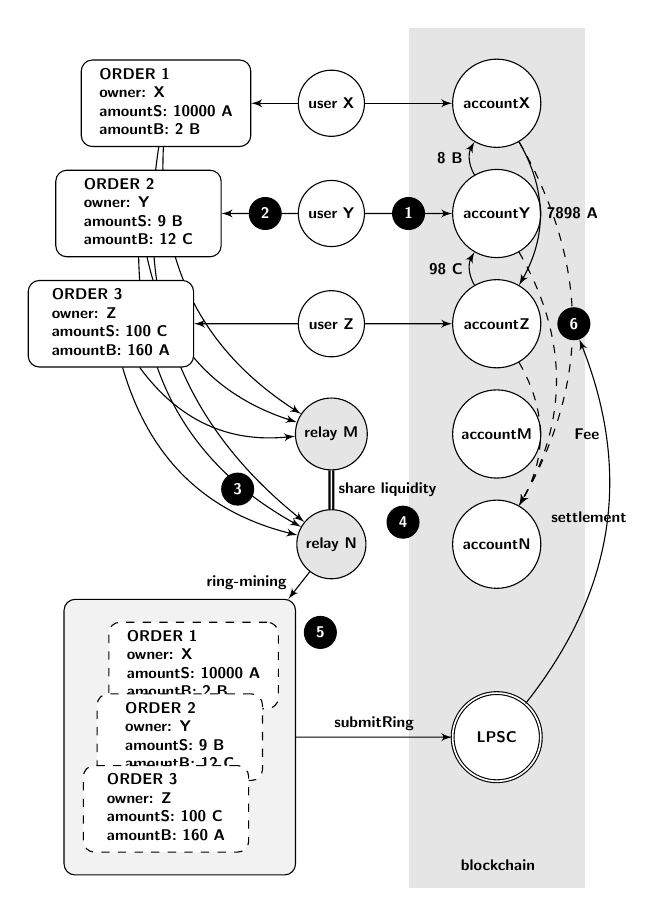
\begin{tikzpicture}[
    auto,
    scale=0.7,
    node distance=2cm,
    >=latex',
    font=\bfseries\footnotesize\sffamily,
    order/.style={
		rectangle,
		scale=0.7,
		rounded corners,
		draw=black,
		text centered,
%		text width=5cm,
		minimum height=12mm,
		minimum width=30mm,
		fill=white
	},
	role/.style={
		circle,
		scale=0.7,
		draw=black,
		text centered,
%		text width=5cm,
		minimum height=12mm,
		minimum width=12mm,
		fill=white
	},
	steps/.style={
		circle,
		scale=0.7,
		draw=black,
		text centered,
%		text width=5cm,
%		minimum height=12mm,
%		minimum width=12mm,
		fill=black,
		text=white
	},
	account/.style={
		circle,
		scale=0.7,
		draw=black,
		text centered,
%		text width=5cm,
		minimum height=16mm,
		minimum width=16mm,
		fill=white
	},
	label/.style={
	  scale=0.7
    }
  ]


 \node [role] (user1)  {user X};
 \node [role, below of=user1] (user2)  {user Y};
 \node [role, below of=user2] (user3)  {user Z};
 \node [role, below of=user3, fill=gray!20] (relay1)  {relay M};
 \node [role, below of=relay1, fill=gray!20] (relay2)  {relay N};


 \node [order, left of=user1, xshift=-1cm] (order1)
 {%
 \begin{tabular}{l}
  \textbf{ORDER 1}\\
  \textbf{owner: X}\\
  \textbf{amountS: 10000 A}\\
  \textbf{amountB: 2 B}
 \end{tabular}
 };

 \draw [draw, ->]  (user1) -- (order1) [label]{};
 \draw [bend right,->] (order1) to node [auto, scale=0.7] {} (relay1);
 \draw [bend right,->] (order1) to node [auto, scale=0.7] {} (relay2);
% \draw [draw, ->]  (order1) |- (relay1) [label]{};
% \draw [draw, ->]  (order1) |- (relay2) [label]{};

 \node [order,left of=user2, xshift=-1.5cm] (order2)
 {%
 \begin{tabular}{l}
  \textbf{ORDER 2}\\
  \textbf{owner: Y}\\
  \textbf{amountS: 9  B}\\
  \textbf{amountB: 12 C}
 \end{tabular}
 };
 \draw [draw, ->]  (user2) -- (order2) [label]{};
 \draw [bend right,->] (order2) to node [auto, scale=0.7] {} (relay1);
 \draw [bend right,->] (order2) to node [auto, scale=0.7] {} (relay2);
% \draw [draw, ->]  (order2) |- (relay1) [label]{};
% \draw [draw, ->]  (order2) |- (relay2) [label]{};
%
\node [order, left of=user3, xshift=-2cm] (order3)
 {%
 \begin{tabular}{l}
  \textbf{ORDER 3}\\
  \textbf{owner: Z}\\
  \textbf{amountS: 100 C}\\
  \textbf{amountB: 160 A}
 \end{tabular}
 };
 \draw [draw, ->]  (user3) -- (order3) [label]{};
 \draw [bend right,->] (order3) to node [auto, scale=0.7] {} (relay1);
 \draw [bend right,->] (order3) to node [auto, scale=0.7] {} (relay2);
% \draw [draw, ->]  (order3) |- (relay1) [label]{};
% \draw [draw, ->]  (order3) |- (relay2) [label]{};

% // The Ring
\node [order,
yshift=-1.5cm,
xshift=-2.75cm,
below of=relay2,
fill=gray!10,
minimum width=4.2cm,
minimum height=5cm] (ring) {};


\node [order, dashed, below of=relay2,yshift=-0.2cm,xshift=-2.5cm] (order11)
 {%
 \begin{tabular}{l}
  \textbf{ORDER 1}\\
  \textbf{owner: X}\\
  \textbf{amountS: 10000 A}\\
  \textbf{amountB: 2 B}
 \end{tabular}
 };
 \node [order, dashed,below of=order11,xshift=-0.25cm,yshift=0.7cm] (order21)
 {%
 \begin{tabular}{l}
  \textbf{ORDER 2}\\
  \textbf{owner: Y}\\
  \textbf{amountS: 9  B}\\
  \textbf{amountB: 12 C}
 \end{tabular}
 };
\node [order, dashed,below of=order21,xshift=-0.25cm,yshift=0.7cm] (order31)
 {%
 \begin{tabular}{l}
  \textbf{ORDER 3}\\
  \textbf{owner: Z}\\
  \textbf{amountS: 100 C}\\
  \textbf{amountB: 160 A}
 \end{tabular}
 };

 % // The blockchain
\node [
rectangle,
fill=gray!20,
right of=user1,
yshift=-4.5cm,
xshift=0.1cm,
scale=0.7,
minimum width=3.2cm,
minimum height=15.6cm] (blockchain) {\parbox[b][15cm]{1.3cm}{blockchain}};
% blockchain accounts
  \node [account, right of=user1, xshift=1cm] (account1)  {accountX};
  \node [account, right of=user2, xshift=1cm] (account2)  {accountY};
  \node [account, right of=user3, xshift=1cm] (account3)  {accountZ};
  \node [account, right of=relay1, xshift=1cm] (account4)  {accountM};
  \node [account, right of=relay2, xshift=1cm] (account5)  {accountN};
  \node [account, double, below of=account5, yshift=-1.5cm] (psc)  {LPSC};

 \draw [draw, ->]  (user1) -- (account1) [label]{};
 \draw [draw, ->]  (user2) -- (account2) [label]{};
 \draw [draw, ->]  (user3) -- (account3) [label]{};
% \draw [draw, ->]  (relay1) -- (account4) [label]{};
% \draw [draw, ->]  (relay2) -- (account5) [label]{};
 \draw [draw, double, thick]  (relay1) to node [auto, scale=0.7] {share liquidity}  (relay2) [label]{};
% \draw [draw, ->]  (relay1) -- (ring) [label]{};
 \draw [draw, ->]  (relay2) to node [auto, scale=0.7, xshift=-1.8cm, yshift=0.3cm] {ring-mining}  (ring) [label]{};
 \draw [draw, ->]  (ring) to node [auto, scale=0.7] {submitRing} (psc) [label]{};

 \draw [bend left,->] (account1) to node [auto, scale=0.7] {\textbf{7898 A}} (account3);
 \draw [bend left,->] (account2) to node [auto, scale=0.7] {\textbf{8 B}} (account1);
 \draw [bend left,->] (account3) to node [auto, scale=0.7] {\textbf{98 C}} (account2);

 \draw [bend left,->, dashed] (account1) to node [auto, scale=0.7] {} (account5);
 \draw [bend left,->, dashed] (account2) to node [auto, scale=0.7] {} (account5);
 \draw [bend left,->, dashed] (account3) to node [auto, scale=0.7, xshift=.5cm] {\textbf{Fee}} (account5);


% \draw [draw,->] (order1) -- node [label] {\textbf{7898 A}} (order3);
% \draw [draw,->] (order2) -| node [label, xshift=-1.8cm] {\textbf{8 B}} (order1);
% \draw [draw,->] (order3) |- node [label, xshift=1cm, yshift=0.24cm] {\textbf{98 C}} (order2);

\node [steps, right of=user2, xshift=-0.6cm] () {1};
\node [steps, left of=user2, xshift=0.8cm] () {2};
\node [steps, left of=relay2, xshift=0.3cm, yshift=1cm] () {3};
\node [steps, left of=relay1, xshift=3.3cm, yshift=-1.6cm] () {4};
\node [steps, below of=relay2, xshift=-0.2cm, yshift=0.4cm] () {5};
\node [steps, right of=account3, xshift=-0.6cm] (step5) {6};

 \draw [bend right, ->]  (psc) to node [auto, scale=0.7, xshift=0.5cm] {settlement} (step5) [label]{};

\end{tikzpicture}

\caption{Quy trình thương mại Loopring }
\label{fig:process}
\end{figure}
\end{center}
%\end{minipage}
\item \textbf{Khai thác vòng (Order Matching):  }Những người khai thác vòng cố gắng lấp đầy các lệnh hoặc một phần theo tỷ giá nhất định hoặc tốt hơn bằng cách kết hợp nó với nhiều lệnh. Khai thác vòng là lý do chính tại sao giao thức có thể cung cấp tính thanh khoản cao cho bất kỳ cặp nào. Nếu tỷ lệ thực hiện tốt hơn so với người dùng Y đã chỉ định, số dư được chia sẻ giữa tất cả các lệnh mua bán trong vòng lệnh. Như là một phần thưởng, người khai thác mỏ chọn giữa phần số dư (Margin-Split, và trả lại LRx cho người dùng), hoặc chỉ đơn giản là giữ lệ phí LRx.

\item \textbf{Sự xác thực và Giải quyết: }Vòng lệnh được nhận bởi LPSC. Nó kiểm tra nhiều lần để xác minh dữ liệu được cung cấp bởi các thợ khai thác vòng và xác định xem có thể giải quyết toàn bộ hay một phần vòng lệnh (phụ thuộc vào tỷ lệ lấp đầy của các lệnh trong vòng và token trong ví của người dùng). Nếu tất cả các kiểm tra đều thành công, hợp đồng sẽ tự động chuyển các token cho người dùng và đồng thời trả phí cho người khai thác mỏ và lệ phí ví. Nếu số dư của người sử dụng Y được xác định bởi LPSC là không đủ, sẽ được coi là thu nhỏ lại: lệnh mà được thu nhỏ sẽ tự động tăng lên kích thước ban đầu nếu tiền được gửi đến địa chỉ của nó đủ, không giống như hủy bỏ, đó là một chiều và không thể đảo ngược.


\end{enumerate}

\section{Vận hành linh hoạt\label{sec:business_model}}
Điều quan trọng cần lưu ý là tiêu chuẩn mở của Loopring cho phép các thành phần có sự linh hoạt đáng kể trong cách hoạt động của chúng. Các thành phần hoạt động được tự do triển khai các mô hình kinh doanh mới và cung cấp giá trị cho người dùng nếu họ chọn. Hệ sinh thái là mô đun và được thiết kế để hỗ trợ sự tham gia của rất nhiều ứng dụng.

\subsection{Bảng đấu giá\label{sec:order_book}}
Các chuyển tiếp có thể thiết kế các bảng đấu giá của chúng bằng bất kỳ cách nào để hiển thị và so khớp các lệnh của người dùng. Đây là lần đầu tiên nó được thiết kế trên mô hình OTC, trong đó lệnh mua bán giới hạn chỉ dựa trên giá. Các dãy Timestamp của lệnh, nói cách khác, không có ảnh hưởng đến bảng đấu giá. Tuy nhiên, một chuyển tiếp là miễn phí để thiết kế các bảng đấu giá của chúng theo cách để tính toán một động cơ phù hợp sàn giao dịch tập trung, nơi mà các lệnh được xếp hạng bằng giá, trong khi vẫn tôn trọng dãy timestamp. Nếu một chuyển tiếpcó thể làm được điều này với bảng đấu giá, chúng có thể sở hữu hay tích hợp một ví, có các lệnh của những ví đó được chuyển riêng lẻ cho từng chuyển tiếp, cái mà có khả năng sẽ phù hợp với lệnh sau này tùy thuộc vào thời gian. Bất cứ cấu hình nào như vậy đều khả thi.
Trong khi Các giao thức sàn giao dịch phân tán DEX vào các thời điểm yêu cầu chuyển tiếp phải có các tài nguyên - token khởi tạo cân bằng để đặt các lệnh -Các chuyển tiếp Loopring cần tìm một lệnh thích hợp để giao dịch, và có thể làm như vậy mà không cần token khởi tạo.

\subsection{Chia sẽ tài nguyên\label{sec:liquidity_sharing}}
Các chuyển tiếp được tự do thiết kế cách họ chia sẻ thanh khoản (đơn đặt hàng) với nhau. Hiệp hội Blockchain của chúng tôi chỉ là một giải pháp cho vấn đề này, và hệ sinh thái được tự do để kết nối và liên lạc. Bên cạnh việc tham gia vào một liên minh blockchain, họ có thể xây dựng và quản lý riêng của mình, tạo ra các quy tắc / ưu đãi khi họ thấy phù hợp. Các chuyển tiếp cũng có thể hoạt động một mình, như trong thực hiện ví nhạy cảm-thời gian. Tất nhiên, có nhiều lợi thế rõ ràng trong việc giao tiếp với các chuyển tiếp khi theo đuổi các tác động của mạng lưới, tuy nhiên các mô hình kinh doanh khác nhau có thể xứng đáng chia sẽ các thiết kế và chia sẽ phí trong nhiều cách.

\section{Chi tiết của giao thức\label{sec:protocol}}
\subsection{Sự mổ xẻ của một lệnh\label{anatomy}}
Một lệnh là một gói dữ liệu mô tả mục đích thương mại của người dùng. Lệnh Loopring được định nghĩa bởi Mô hình lệnh một hướng hay còn gọi là UDOM, như sau:
\begin{small}
\begin{verbatim}
 message Order {
    address protocol;
    address owner;
    address tokenS;
    address tokenB;
    uint256 amountS;
    uint256 amountB;
    unit256 lrcFee
    unit256 validSince; // Seconds since epoch
    unit256 validUntil; // Seconds since epoch
    uint8   marginSplitPercentage;  // [1-100]
    bool    buyNoMoreThanAmountB;
    uint256 walletId;
    // Dual-Authoring address
    address authAddr;
   	// v, r, s are parts of the signature
    uint8   v;
    bytes32 r;
    bytes32 s;
    // Dual-Authoring private-key,
    // not used for calculating order's hash,
    // thus it is NOT signed.
    string  authKey;
  }
\end{verbatim}
\end{small}
Để đảm bảo nguồn gốc của các lệnh, nó được ký kết chống lại các hash của các tham số của nó, không bao gồm authAddr, với mã khóa riêng của người dùng. Tham số authAddr được sử dụng cho việc ký các vòng lệnh mà lệnh đó là một phần trong đó, ngăn chặn lỗi chạy trước. Vui lòng tham khảo mục 9.1 để biết thêm chi tiết. Chữ ký được biểu diễn bởi các trường v, r, và các s, được bao gồm trong các tham số lệnh thông qua mạng. Điều này đảm bảo lệnh đó vẫn không thay đổi trong suốt cả thời gian. Mặc dù lệnh không bao giờ thay đổi, giao thức này vẫn có thể được tính trạng thái hiện tại của nó dựa vào sự cân bằng của địa chỉ của nó theo với các biến khác.
UDOM không bao gồm một giá (mà phải là một số điểm nổi theo tự nhiên), nhưng thay vào đó sử dụng tỷ giá hoặc r, được thể hiện bằng số lượng S / số lượng B. Giá đó không phải là một số điểm nổi, nhưng nó biểu hiện sẽ chỉ có thể thực hiện với các số nguyên chưa được ký khác trên mệnh lệnh, để giữ tất cả các kết quả trung gian như các số nguyên chưa được ký và làm tăng độ chính xác tính toán.

\subsubsection{Khối lượng mua}
Khi một vòng thợ khai thác vòng trùng khớp với các lệnh, có khả năng một giá tốt hơn sẽ được thực thi, cho phép người sử dụng nhận được nhiều token B hơn là họ xác định. Tuy nhiên, nếu Mua không quá số lượng B buyNoMoreThanAmountB được đặt thành True, giao thức đảm bảo nhựgười dùng nhận được không nhiều hơn số lượng B của tokenB. Do đó, tham số Mua không quá số lượng B của UDOM xác định khi một lệnh hoàn toàn được lấp đầy. Mua không quá số lượng B áp dụng giới hạn về số lượng S hoặc số lượng B, và cho phép người dùng thể hiện các ý định thương mại chi tiết hơn các lệnh mua / bán truyền thống.
Ví dụ: với amountS = 10 và amountB = 2, tỷ lệ r = 10/2 = 5. Do đó người dùng sẵn sàng bán 5 token S cho mỗi token B. Vòng khai thác trùng khớp và tìm tỷ lệ người dùng là 4, cho phép người dùng nhận được 2,5 tokenB thay vì 2. Tuy nhiên, nếu người dùng chỉ muốn 2 tokenB và đặt cờ Mua không quá số lượng B  thành hiện thực, LPSC sẽ thực hiện giao dịch với tỷ lệ của 4 và người dùng bán 4 tokenS cho mỗi tokenB, tiết kiệm hiệu quả 2 tokenS. Lưu ý rằng điều này không tính đến chi phí khai thác tài khoản (Xem phần 8.1).

Thật vậy, nếu chúng ta sử dụng

\begin{verbatim}
	      Order(amountS,tokenS,
	            amountB,tokenB,
	            buyNoMoreThantokenB)
\end{verbatim}
Để thể hiện một lệnh ở dạng đơn giản, sau đó cho thị trường ETH / USD trên một sàn giao dịch truyền thống, mô hình mua bán truyền thống có thể thể hiện thứ tự 1 và thứ 3 dưới đây, nhưng không phải là hai:

\begin{enumerate}
	\item Bán 10 ETH với giá 300 USD / ETH. Lệnh này có thể được biểu diễn bằng:  \verb|Order(10, ETH, 3000, USD, False)|.
	\item Bán ETH với giá 300 USD / ETH để được 3000 USD. Lệnh này có thể được biểu diễn như sau:  \verb|Order(10, ETH, 3000, USD, True)|.
	\item Mua 10 ETH với giá 300 USD / ETH, lệnh này có thể được thể hiện bằng:   \verb|Order(3000, USD, 10, ETH, True)|.
	\item Chi tiêu 3000 USD để mua càng nhiều ETH càng tốt ở mức 300 USD / ETH: \verb|Order(3000, USD, 10, ETH, False)|.
\end{enumerate}

\subsection{Xác thực vòng\label{sec:ring_verification}}
Hợp đồng Thông minh Loopring không phải được thể hiện tính toán tỷ giá giao dịch và số lượng, nhưng phải nhận và xác minh những gì những người khai thác vòng cung cấp cho các giá trị này. Các tính toán này được thực hiện bởi những người khai thác vòng vì hai lý do chính: (1) ngôn ngữ lập trình cho các hợp đồng thông minh, chẳng hạn như tính vững chắc [19] trên Ethereum, không có hỗ trợ cho toán học điểm nổi, đặc biệt là pow (x, 1 / n) (tính gốc rễ thứ n của một số điểm nổi), và (2) nó là mong muốn cho việc tính toán được thực hiện off-line để giảm bớt tính toán và chi phí blockchain.

\subsubsection{Kiểm tra vòng phụ \label{sec:sub_ring_check}}
Bước này ngăn cản các đầu cơ hưởng chênh lệch bất hợp pháp thực hiện tất cả các giao dịch ký quỹ trong một vòng lệnh bằng cách thực hiện các lệnh mới mới bên trong nó. Về cơ bản, một khi vòng lệnh hợp lệ được tìm thấy bởi một người khai thác vòng, có thể sẽ bị cám dỗ để thêm các lệnh vào vòng lệnh để thu đầy đủ giao dịch ký quỹ của người dùng (đánh giá mức chiết khấu). Theo tính toán của hình 3, cẩn thận tính x1, y1, x2 và y2 sẽ làm cho sản phẩm của tất cả các lệnh sẽ được chính xác những gì bạn cần.
\begin{center}
\begin{figurehere}
\centering
\tikzstyle{block} = [draw, fill=blue!20, rectangle,
    minimum height=3em, minimum width=6em]
\tikzstyle{sum} = [draw, fill=blue!20, circle, node distance=1cm]
\tikzstyle{input} = [coordinate]
\tikzstyle{output} = [coordinate]
\tikzstyle{pinstyle} = [pin edge={to-,thin,black}]

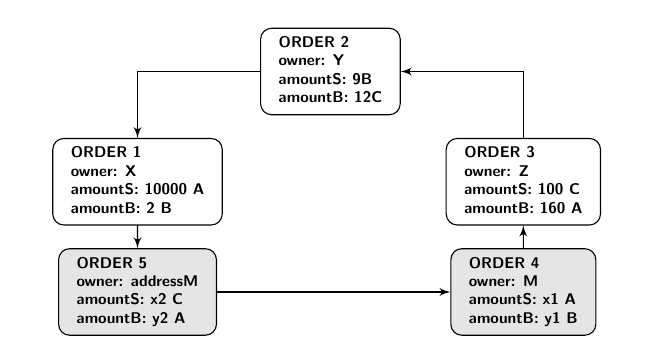
\begin{tikzpicture}[
    auto,
    node distance=2cm,
    >=latex',
    font=\bfseries\footnotesize\sffamily,
    order/.style={
		scale=0.7,
		rectangle,
		rounded corners,
		draw=black,
		text centered,
%		text width=5cm,
		minimum height=12mm,
		fill=white
	},
	label/.style={
		scale=0.7
	}
  ]
    % We start by placing the blocks

  \node [order] (order2)
 {%
 \begin{tabular}{l}
  \textbf{ORDER 2}\\
  \textbf{owner: Y}\\
  \textbf{amountS: 9B}\\
  \textbf{amountB: 12C}
 \end{tabular}
 };

  \node [order, below of=order2, xshift=-3.5cm] (order1)
 {%
 \begin{tabular}{l}
  \textbf{ORDER 1}\\
  \textbf{owner: X}\\
  \textbf{amountS: 10000 A}\\
  \textbf{amountB: 2 B}
 \end{tabular}
 };


  \node [order, below of=order2, xshift=3.5cm] (order3)
 {%
 \begin{tabular}{l}
  \textbf{ORDER 3}\\
  \textbf{owner: Z}\\
  \textbf{amountS: 100 C}\\
  \textbf{amountB: 160 A}
 \end{tabular}
 };

   \node [order, below of=order3, fill=gray!20] (order4)
 {%
 \begin{tabular}{l}
  \textbf{ORDER 4}\\
  \textbf{owner: M}\\
  \textbf{amountS: x1 A}\\
  \textbf{amountB: y1 B}
 \end{tabular}
 };


  \node [order, below of=order1, fill=gray!20] (order5)
 {%
 \begin{tabular}{l}
  \textbf{ORDER 5}\\
  \textbf{owner: addressM}\\
  \textbf{amountS: x2 C}\\
  \textbf{amountB: y2 A}
 \end{tabular}
 };

 \draw [draw,->] (order1) -- node [label, xshift=-2cm] {} (order5);
 \draw [draw,->] (order2) -| node [label, xshift=-1.6cm] {} (order1);
 \draw [draw,->] (order3) |- node [label, xshift=1cm] {} (order2);
 \draw [draw,->] (order4) -- node [label, xshift=1.8cm] {} (order3);
 \draw [draw,->] (order5) -- node [label, yshift=0.2cm] {} (order4);

\end{tikzpicture}

\caption{Một vòng lệnh với một vòng phụ}
\label{fig:subring}
\end{figurehere}
\end{center}
Đây là Rủi ro không, giá trị không được thêm vào mạng, và được coi là sự điều khiển không công bằng cho người khai thác vòng. Để ngăn chặn điều này, Loopring yêu cầu một vòng lặp hợp lệ không thể chứa bất kỳ vòng phụ. Để kiểm tra điều này, LPSC đảm bảo một token không thể đặt ở một vị trí mua hay bán hai lần. Trong sơ đồ trên, chúng ta có thể thấy rằng token A là một token bán hai lần và mua hai lần, điều mà sẽ không được phép.

\subsubsection{Kiểm tra tỷ lệ lấp đầy\label{sec:fill_rate_check}}
Việc tính tỷ giá hối đoái trong vòng lệnh được thực hiện bởi người khai thác vòngvì lý do nêu trên. Đó là LPSC phải xác minh là đúng. Thứ nhất, nó xác nhận rằng tỷ lệ mua mà người khai thác vòng có thể thực hiện cho từng lệnh là bằng hoặc ít hơn tỷ giá mua ban đầu được đặt bởi người dùng. Điều này đảm bảo rằng người dùng được tỷ giá giao dịch tối thiểu mà họ yêu cầu hoặc tốt hơn. Một khi các tỷ giá hối đoái được xác nhận, LPSC đảm bảo rằng mỗi tỷ giá hối đoái trong vòng lệnh chia sẽ chiết khấu tỷ giá tương tự. Ví dụ, nếu tỷ lệ chiết khấu là $\gamma$, thì giá cho mỗi lệnh sẽ là:

$r_{0\rightarrow 1} \cdot (1-\gamma)$, $r_{1\rightarrow 2} \cdot (1-\gamma)$, $r_{2 \rightarrow 0} \cdot (1-\gamma)$, và thõa mản:
\begin{equation}
r_{0\rightarrow 1} \cdot (1-\gamma)\cdot r_{1\rightarrow 2} \cdot (1-\gamma) \cdot r_{2 \rightarrow 0} \cdot (1-\gamma) = 1
\end{equation}
Do đó:
\begin{equation}
\gamma = 1- \frac{1}{\sqrt[3]{r_{0\rightarrow 1} \cdot r_{1\rightarrow 2} \cdot r_{2\rightarrow 0}}}\text{.}
\end{equation}
Nếu giao dịch với qua n lệnh, chiết khấu sẽ là:
\begin{equation}
\gamma = 1- \frac{1}{\sqrt[n]{\prod_{i=0}^{n-1} r^i}} \text{,}
\end{equation}

Khi $r^i$   là tỷ lệ doanh số đặt lệnh mua bán của lệnh thứ $i$. Rõ ràng, chỉ khi tỷ lệ chiết khấu là $\gamma \ge 0$,những lệnh này có thể được lấp đầy; và tỷ giá hối đoái thực tế của lệnh thứ $\hat{r^i} = r^i \cdot (1-\gamma)$, $\hat{r^i}\le r^i$.

Trở lại ví dụ lúc nãy, khi mà Alice có 15 token A và muốn 4 token B, Bob có 10 token B và muốn 30 token A. Nếu lấy token A làm tham chiếu, sau đó Alice mua token B với giá $\frac{15}{4}$ = 3.75A, trong khi Bob bán token B với giá 3.00A. Để tính toán chiết khấu: $\frac{150}{120}$ = 1.25 do vậy $\frac{1}{1.25}$ = 0.8 = $(1 - \gamma)^2$. Do đó, tỷ giá trao đổi hoàn lại giao dịch công bằng cho cả 2 bên là: $\sqrt{0.8}\cdot 3.75 \approx 3.3541$ token A cho mỗi token B. Bob cho 4 token B và nhận được 13.4164 token A, nhiều hơn con số 12 mà anh ta mong đợi cho 4 token này. Alice nhận 4 token B như dự định nhưng chỉ cho 13.4164 A, ít hơn con số 15 token mà cô đã sẵn sàng cung cấp 4 token B. Lưu ý, một phần lợi nhuận này sẽ được áp dụng để thanh toán các khoản phí để khuyến khích các thợ mỏ (và ví).8.1).

\subsubsection{Theo dõi và hủy lấp đầy}
Một người dùng có thể hủy hoàn toàn hoặc một phần của một lệnh bằng cách gửi một giao dịch đặc biệt đến LPSC, chứa các chi tiết về lệnh đó và số lượng cần hủy. LPSC đưa nó vào tài khoản, lưu trữ số lượng cần dừng và tạo ra một dữ kiện OrderCancelled đến mạng. LPSC giữ theo dõi các số lượng đã được lấp đầy hay đã hủy bằng việc lưu trữ các giá trị của chúng sử dụng hash của lệnh như một định danh. Dữ liệu này có thể truy cập công khai và sự kiện OrderCancelled/ OrderFilled được phát khi nó thay đổi.  Theo dõi các giá trị này là rất quan trọng đối với LPSC trong suốt các bước giải quyết vòng lệnh.
 	LPSC cũng hỗ trợ hủy tất cả các lệnh cho bất kỳ cặp giao dịch nào với sự kiện hủy lệnh OrderCancelled và hủy tất cả các lệnh cho một địa chỉ với sự kiện AllOrdersCancelled.

\subsubsection{Thước đo lệnh\label{sec:order_scaling}}
Các lệnh được tỷ lệ theo lịch sử của các tài khoản đã được lấp đầy hoặc đã hủy và số dư tài khoản hiện tại. Quá trình tìm ra lệnh với số lượng nhỏ nhất có thể được lấp đầy dựa vào các đặc tính và sử dụng nó như một tham khảo để chia tỷ lệ cho tất cả các giao dịch trong vòng lệnh.

Tìm lệnh có giá trị thấp nhất có thể giúp bạn tìm ra khối lượng cho mỗi lệnh. Ví dụ, nếu lệnh thứ i là lệnh có giá trị thấp nhất, thì số lượng của token đã được bán từ mỗi lệnh sˆ và số lượng token đã được mua ˆb  từ mỗi lệnh có thể tính toán:
\[
\begin{split}
&\hat{s}^{i}=\overline{s}_i\text{, } \hat{b}^{i}=\hat{s}^{i}/ \hat{r}^i\text{, }\text{;}\\
&\hat{s}^{i\oplus 1}=\hat{b}^i\text{, } \hat{b}^{i\oplus 1}=\hat{s}^{i\oplus 1}/ \hat{r}^{i\oplus 1}\text{;}\\
&\hat{s}^{i\oplus 2}=\hat{b}^{i\oplus 1}\text{, } \hat{b}^{i\oplus 2}=\hat{s}^{i\oplus 2}/ \hat{r}^{i\oplus 2}\text{;}\\
& ...
%\text{.}
\end{split}
\]
Với     si   là số dư còn lại khi lệnh đã được lấp đầy một nửa.
Trong quá trình thực hiện chúng ta có thể giả định một cách an toàn bất kỳ lệnh nào trong vòng lệnh cógiá trị thấp nhất, sau đó lặp qua vòng lệnh nhiều nhất hai lần để tính toán khối lượng lấp đầy của mỗi lệnh.
Ví dụ: Nếu số tiền nhỏ nhất được so sánh với lệnh ban đầu là 5\%, tất cả các giao dịch trong vòng lệnh được thu nhỏ xuống 5\%. Một khi các giao dịch được hoàn thành thì lệnh đó được xem là có số lượng nhỏ nhất còn lại để được lấp đầy.

\subsection{Thỏa thuận vòng\label{sec:settlement}}
Nếu vòng lệnh hoàn thành tất cả các kiểm tra trước đó, vòng lệnh có thể đóng và có thể thực hiện các giao dịch. Điều này có nghĩa là tất cả n lệnh đều được đóng vòng lệnh, kết nối như trong hình 4:
\begin{center}
\begin{figurehere}
\centering
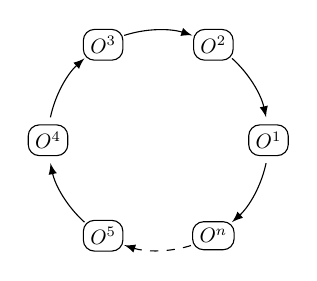
\begin{tikzpicture}[
circle/.style={
		scale=0.75,
		rounded corners,
		draw=black,
		text centered,
		}
]

\def \n {6}
\def \m {4}
\def \radius {1.4cm}
\def \margin {12} % margin in angles, depends on the radius

\foreach \s in {1,...,\m}
{
  \node[draw, circle] at ({360/\n * (\s - 1)}:\radius) {$O^\s$};
  \draw[<-, >=latex] ({360/\n * (\s - 1)+\margin}:\radius)
    arc ({360/\n * (\s - 1)+\margin}:{360/\n * (\s)-\margin}:\radius);
}

\node[draw, circle] at ({360/\n * 4}:\radius) {$O^5$};
  \draw[<-, dashed, >=latex] ({360/\n * 4+\margin}:\radius)
    arc ({360/\n * 4+\margin}:{360/\n * (5)-\margin}:\radius);

\node[draw, circle] at ({360/\n * 5}:\radius) {$O^n$};
  \draw[<-, >=latex] ({360/\n * 5+\margin}:\radius)
    arc ({360/\n * 5+\margin}:{360/\n * (6)-\margin}:\radius);


\end{tikzpicture}
\caption{thỏa thuận vòng}
\label{fig:settlement}
\end{figurehere}
\end{center}
Để thực hiện giao dịch, LPSC sử dụng hợp đồng thông minh TokenTransferDelegate, làm cho giao thức trở nên dễ nâng cấp hơn vì tất cả các lệnh chỉ cần ủy quyền cho đại diện này khác với các phiên bản khác của giao thức.
Đối với mỗi lệnh trong vòng lệnh, một thanh toán của token S được thực thi đến lệnh trước hay kế tiếp tùy thuộc vào việc thực thi. Sau đó, phí khai thác vòng được thanh toán tùy thuộc vào mô hình tính phí do người khai thác vòng chọn. Cuối cùng, tất cả các giao dịch được thực hiện, một sự kiện RingMined được phát ra.

\subsubsection{Các sự kiện được phát\label{sec:events}}
Giao thức này phát ra các sự kiện cho phép chuyển tiếp, các trình duyệt lệnh và các tác nhân khác nhận lệnh càng sớm càng tốt. Các sự kiện được phát ra là:
\begin{itemize}
	\item \textbf{OrderCancelled}: Một lệnh cụ thể bị hủy.
	\item \textbf{OOrdersCancelled}: Tất cả các lệnh của một cặp giao dịch từ một địa chỉ sỡ hữu bị hủy.  cancelled.
	\item \textbf{AllOrdersCancelled}: Tất cả các lệnh của các cặp giao dịch từ một địa chỉ sỡ hữu bị hủy.
	\item \textbf{RingMined}: Một vòng lệnh đã được thiết lập thành công. Sự kiện này chứa dữ liệu liên quan tới mỗi  giao dịch token vòng trong.
\end{itemize}

\section{LRx Token\label{sec:token}}
LRx là ký hiệu dấu hiệu tổng quát của chúng tôi. LRC là mã thông báo Loopring trên Ethereum, LRQ trên Qtum và LRN trên NEO, v.v. Các loại LRx khác sẽ được giới thiệu trong tương lai.

\subsection{Mô hình phí\label{sec:fee_model}}
Khi người dùng tạo ra một lệnh, họ chỉ định số tiền thanh toán cho người khai thác vòng như là phí, cùng với tỷ lệ phần trăm của lợi nhuận (marginSplitPercentage) theo lệnh mà người khai thác vòng có thể yêu cầu bồi thường. Đây được gọi là phân chia lợi nhuận. Quyết định lựa chọn phí hay tỷ lệ phần trăm lợi nhuận là do người khai thác vòng chọn.

Một ví dụ của sự phân chia lợi nhuận:
\begin{center}
\begin{figurehere}
\centering
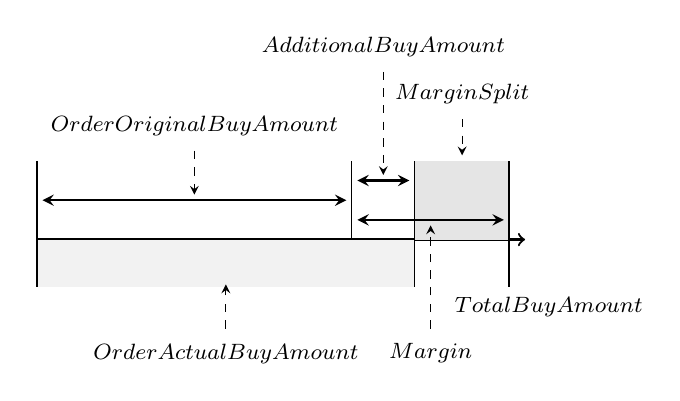
\begin{tikzpicture}[
scale=1,
font=\bfseries\footnotesize\sffamily,
classical/.style={thick,<->,shorten >=2pt,shorten <=2pt,>=stealth},
oneway/.style={->,dashed,shorten >=2pt,shorten <=2pt,>=stealth}
]
    % Draw axes
    \draw [->,thick] (0,1) node (yaxis) [above] {$$}
        |- (6.2,0) node (xaxis) [right] {$$};

    \draw
  	(4,0) coordinate (A)
  	(4,1) coordinate (A2)
  	(4.8,-0.6) coordinate (B)
  	(4.8,1) coordinate (B2)
  	(6,-0.6) coordinate (C)
  	(6,1) coordinate (C2);
  	
  	\fill [draw=none, fill=gray!20]
    (4.8, 0) rectangle (6, 1);

  	\fill [draw=none, fill=gray!10]
    (0, -0.6) rectangle (4.8, 0);

	\draw[thick] (0, -0.6) -- (0, 0.6) node[below]{$$};
  	\draw[thick, thin] (A) -- (A2) node[below]{$$};
  	\draw[thick, thin] (B) -- (B2) node[below]{$$};
  	\draw[thick] (C) node[below, xshift=0.5cm]{$Total Buy Amount$} -- (C2) ;
  	
  	\draw[classical] (0, 0.5) -> (4, 0.5) node[below]{$$};
  	\draw[classical] (4, 0.75) -> (4.8, 0.75) node[below]{$$};
%  	\draw[classical] (4.8, 0.5) -> (6, 0.5) node[below]{$$};
  	\draw[classical] (4, 0.25) -> (6, 0.25) node[below]{$$};

  	
  	\draw[oneway] (2, 1.2) node[above]{$Order Original Buy Amount$} -- (2, 0.5);
  	\draw[oneway] (4.4, 2.2) node[above]{$Additional Buy Amount$} -- (4.4, 0.75);
  	\draw[oneway] (5.4, 1.6) node[above]{$Margin Split$} -- (5.4, 1);
  	\draw[oneway] (5, -1.2) node[below]{$Margin$} -- (5, 0.25);
  	\draw[oneway] (2.4, -1.2) node[below]{$Order Actual Buy Amount$} -- (2.4, -0.5);



\end{tikzpicture}
\caption{chia 60\% giao dịch ký quỹ}
\label{fig:marginsplit}
\end{figurehere}
\end{center}

Nếu ký quỹ là quá nhỏ, một thợ khai thác vòng sẽ chọn lệ phí LRx. Nếu ngược lại, giao dịch ký quỹ đủ lớn để phân chia mà thu được nhiều hơn  phí LRx, thì một nhà người khai thác vòng sẽ chọn phân chia ký quỹ. Tuy nhiên, có một điều kiện khác: khi người khai thác vòng chọn phân chia ký quỹ, họ phải trả cho người sử dụng (người đặt lệnh) một khoản phí, bằng LRx mà người sử dụng sẽ phải trả cho người khai thác vòng như một khoản phí bằng với phí LRx người dùng sẽ phải trả cho người khai thác vòng như là phí giao dịch. Điều này làm tăng ngưỡng của người khai thác vòng sẽ chọn phân chia ký quỹ
Để gấp đôi phí LRx của lệnh, tăng khuynh hướng chọn lựa phí LRx. Điều này cho phép những người khai thác vòng thu được thu nhập liên tục trên các lệnh có tỷ suất ký quỹ thấp để đánh đổi thu nhập ít hơn trên vòng lệnh ký quỹ cao hơn. Mô hình tính phí của chúng tôi kỳ vọng rằng khi thị trường tăng trưởng và chín muồi, sẽ có ít hơn các vòng lệnh ký quỹ cao, do đó cần phải có phí LRx cố định để khuyến khích.

Chúng tôi kết luận với biểu đồ bên dưới:
\begin{center}
\begin{figurehere}
\centering
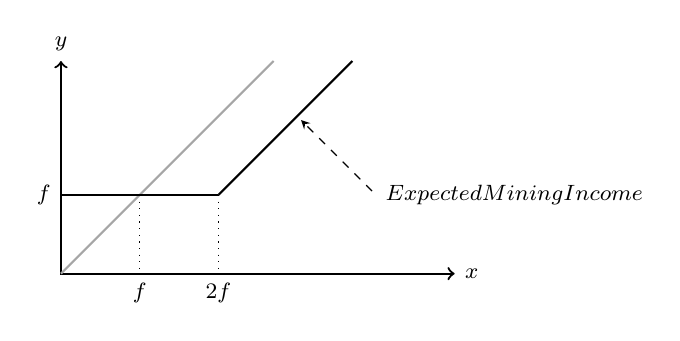
\begin{tikzpicture}[
font=\bfseries\footnotesize\sffamily,
oneway/.style={->,dashed,shorten >=2pt,shorten <=2pt,>=stealth},
scale=1]
    % Draw axes
    \draw [<->,thick] (0,2.7) node (yaxis) [above] {$y$}
        |- (5,0) node (xaxis) [right] {$x$};

    \draw
  	(1,1) coordinate (A)
  	(2,1) coordinate (B);
  	
  	
  	\draw[thick] (B) -- (3.7,2.7);
  	\draw[dotted] (B) -- (2,0) node[below] {$2f$};
  	\draw[dotted] (A) -- (1,0) node[below] {$f$};
  	\draw[thick,color=gray!70] (0,0) -- (2.7,2.7);
  	\draw[thick] (0,1) node[left] {$f$}--(B) node[     ]{$$};
 	\draw[oneway] (4,1) node[right]{$Expected Mining Income$} -- (3, 2);


\end{tikzpicture}
\caption{Mô hình phí của Loorping}
\label{fig:feemodel}
\end{figurehere}
\end{center}

Với $ f $ là phí LRx, $ x $ là chia ký quỹ, $ y $ là thu nhập từ việc khai thác.  $y=max(f, x-f)$ như được chỉ thị bởi đường tô đậm; Nếu phí LRx cho một lệnh là 0, phương trình là $y=max(0, x - 0)$ đơn giản hóa đến $y=x$ như được chỉ ra bởi dòng màu xám.

Kết quả là:
\begin{enumerate}
	\item Nếu phân chia ký quỹ là 0, người khai thác vòng sẽ chọn mức phí trần LRx mà vẫn được khuyến khích.
	\item Nếu phí LRx là 0, kết quả dòng màu xám và thu nhập được dựa trên một mô hình tuyến tính chung.
	\item Khi thu nhập từ chia ký quỹ lớn hơn 2 lần phí LRx thì người khai thác vòng sẽ chọn chia ký quỹ và trả phí LRx cho người dùng.
\end{enumerate}
Cần lưu ý rằng nếu phí LRx là khác không, cho dù các thợ khai thác vòng chọn lựa chọn nào thì sẽ luôn luôn có một chuyển đổi phí LRx giữa người khai thác vòng và người gửi lệnh.Một là người khai thác vòng thu được phí LRx hoặc trả phí LRx cho người gửi nếu lấy phí chia ký quỹ.

Những người khai thác vòng sẽ chia sẻ một tỷ lệ nhất định lệ phí với các ví. Khi người dùng đặt một lệnh thông qua một ví và được lấp đầy, ví sẽ được nhận một phần của lệ phí LRx hay chia ký quỹ. Mặc dù đây là mô đun, và mô hình kinh doanh độc đáo hay sự thực hiện được là điều có thể, ý định của chúng tôi là dành cho ví để nhận khoảng 20\% -25\% lệ phí thu được. Ví là một mục tiêu ưu tiên cho liên hợp giao thức Loorping vì họ có cơ sở người dùng nhưng nhỏ hoặc không có nguồn thu nhập.

\subsection{Quản trị phân cấp}
Tại vấn đề cốt lõi, giao thức Loopring là một giao thức xã hội theo nghĩa nó dựa vào sự phối hợp giữa các thành viên để hoạt động hiệu quả theo hướng mục tiêu. Điều này giống với các giao thức cryptoeconomic lớn, và thực tế, tính hữu ích của nó phần lớn được bảo vệ bởi cùng một cơ chế của các vấn đề phối hợp [20], cân bằng kích hoạt mạnh mẽ  và tính hợp lý bị giới hạn. Để kết thúc điều này, các token LRx không chỉ được sử dụng để trả phí, mà còn để sắp xếp các ưu đãi tài chính của các thành viên mạng khác nhau. Sự liên kết như vậy là cần thiết để áp dụng rộng rãi cho bất kỳ giao thức nào, nhưng đặc biệt cấp tính đối với các giao thức trao đổi, vì thành công đó chủ yếu dựa vào việc cải thiện tính thanh khoản trong một hệ sinh thái phân tán mạnh mẽ.
Các token LRx sẽ được sử dụng để thực hiện cập nhật các giao thức thông qua sự quản lý phân quyền. Việc cập nhật hợp đồng thông minh sẽ được quản lý bởi các chủ sở hữu token để đảm bảo tính liên tục và an toàn, đồng thời giảm thiểu rủi ro của thanh khoản bị siết lại thông qua sự không tương thích. Do các hợp đồng thông minh không thể bị thay đổi khi triển khai, có nguy cơ dApps hoặc người dùng cuối tiếp tục tương tác với các phiên bản không dùng nữa và không cho phép họ cập nhật hợp đồng. Khả năng nâng cấp là rất quan trọng đối với thành công của giao thức vì nó phải thích ứng với nhu cầu của thị trường và các blockchains bên dưới. Quản lý phân quyền bởi các bên liên quan của LRx sẽ cho phép cập nhật hợp đồng thông minh hợp đồng mà không làm gián đoạn dApps hoặc người dùng cuối hoặc dựa quá nhiều vào việc trừu tượng hợp đồng thông minh. Số lượng token LRx là cố định , và trong trường hợp của LRC, một phần trăm nhất định bị đóng băng từ quỹ của Loopring và được phân bổ cho các quỹ dự định của cộng đồng

Tuy nhiên, người người sở hữu LRx không phải là các bên liên quan duy nhất để xem xét trong việc định hướng giao thức: các chuyển tiếp / người khai thác vòng, ví, nhà phát triển, và những người khác là một phần không thể tách rời của hệ sinh thái và tiếng nói của họ phải được lắng nghe. Trong thực tế, cho rằng các thành phần này không cần phải giữ bất kỳ LRx để thực hiện vai trò của họ (vì các nhà hoạch định truyền thống / nhà hoạch định thị trường không tồn tại, dự trữ token ban đầu là không bắt buộc) chúng ta phải cho phép các phương pháp thay thế cho lợi ích cần được tôn trọng. Hơn nữa, "đơn giản" bỏ phiếu tokenbased, cả trên on chain và off chain, là một sự giải quyết không hoàn hảo cho việc không đồng ý, như những người bỏ phiếu thấp và quyền sở hữu token tập trung đặt ra những rủi ro. Như vậy, mục đích là để thực hiện một mô hình quản trị được xây dựng theo các lớp, và dựa trên một chia sẻ kiến thức rằng một số quy trình ra quyết định là tiêu chuẩn. Điều này có thể được tạo điều kiện bởi các tổ chức phối hợp cung cấp tín hiệu từ một tập hợp đa dạng của người tham gia, và có lẽ, từ các đầu mối giao thức được thiết lập trước. Do vậy, Loopring sẽ không tránh khỏi việc từ các nhà phát triển giao thức thành người quản lý giao thức.
\section{Phòng chống gian lận và tấn công}

\subsection{Ngăn ngừa lỗi chạy trước Front-running \label{sec:dual_authoring}}
Trong các sàn giao dịch phi tập trung, lỗi chạy trước là khi ai đó cố gắng sao chép giải pháp giao dịch của một nút khác và khai thác nó trước khi giao dịch ban đầu đang nằm trong vùng giao dịch đang chờ xử lý (mempool). Điều này có thể đạt được bằng cách chỉ định mức phí giao dịch cao hơn (giá gas). Vấn đề chính của lỗi chạy trước trong Loopring (và bất kỳ giao thức nào đối với khớp lệnh) là lệnh-filch: khi một người chạy trước đánh cắp một hoặc nhiều lệnh từ một giao dịch vòng lệnh đang chờ xử lý; và, cụ thể cho Loopring: khi một người chạy trước đánh cắp toàn bộ vòng lệnh từ một giao dịch đang chờ xử lý.

Khi một giao dịch vòng không được xác nhận và vẫn ở trong vùng giao dịch đang chờ xử lý, bất kỳ ai cũng có thể dễ dàng phát hiện ra một giao dịch như vậy và thay thế địa chỉ người khai thác minerAddress bằng địa chỉ riêng của họ (filcherAddress), sau đó họ có thể ký lại payload với filcherAddress để thay thế lệnh- dấu hiệu của vòng. Họ có thể đặt giá gas cao hơn và gửi một giao dịch mới với hy vọng rằng người khai thác vòng sẽ chọn giao dịch mới của mình vào khối tiếp theo thay vì giao dịch gốc.

Các giải pháp trước đây cho vấn đề này có những nhược điểm quan trọng: yêu cầu nhiều giao dịch hơn và vì vậy gây tốn nhiều phí cho các thợ khai thác mỏ; và lấy ít nhất hai lần khối để giải quyết một đlệnh. Giải pháp mới của chúng tôi, Dual Authoring [21], bao gồm cơ chế thiết lập hai lần ủy quyền cho các lệnh mua bán - một cho giải quyết, và một cho khai thác vòng.

Quy trình Uỷ quyền hai lần:
\begin{enumerate}

	\item Đối với mỗi lệnh, phần mềm ví sẽ tạo ra một mã khóa công khai / mã khóa cá nhân ngẫu nhiên và đặt cặp khóa vào đoạn mã JSON của lệnh. (Một thay thế sử dụng địa chỉ có được chia ra từ khoá công khai thay vì bản thân khoá đó để giảm kích thước byte. Chúng tôi sử dụng authAddr để biểu diễn một địa chỉ như vậy, và authKey đại diện cho mã khóa riêng của authAddr).

	\item Tính toán hash của lệnh với tất cả các trường trong lệnh đó ngoại trừ r,  v,  s,  và  authKey, và ký hash sử dụng mã khóa cá nhân của người sở hữu (không phải authKey).

	\item Ví sẽ gửi lệnh với authKey để chuyển tiếp cho việc khai thác vòng. Những người khai thác vòn sẽ xác thực rằng authKey và authAddr là được ghép cặp chính xác và chữ ký của lệnh là có giá trị với theo địa chỉ người sỡ hữu.

	\item Khi một vòng lệnh được xác định, người khai thác vòng sẽ sử dụng một authKey của mỗi lệnh để đánh dấu hash của vòng, minerAddress, và tất cả các thông số khai thác. Nếu một vòng lệnh chứa n lệnh, sẽ có n chữ ký bởi n authKeys.  Chúng tôi gọi các chữ ký này là authSignatures.  Người khai thác vòng có thể cần ký hash của vòng cùng nhau với tất cả các thông số đào sử dụng mã khóa riêng của địa chỉ người khai thác minerAddress.

	\item Người khai thác vòng gọi hàm submitRing với tất cả các tham số, cũng như tất cả các authSignatures phụ. Lưu ý rằng authKeys KHÔNG phải là một phần của giao dịch On-chain và do đó vẫn chưa được biết đối với các bên khác với chính bản thân người khai thác vòng.


	\item Giao thức Loopring bây giờ sẽ xác minh mỗi authSignature với authAddr tương ứng đối với mỗi lệnh và từ chối vòng lệnh nếu bất kỳ authSignature nào bị thiếu hoặc không hợp lệ.

\end{enumerate}
Kết quả là:
\begin{itemize}

	\item  Chữ ký của lệnh (bằng mã khóa riêng của địa chỉ người sỡ hữu) đảm bảo rằng lệnh không thể sửa đổi, bao gồm địa chỉ authAddr.
	\item  Chữ ký Người khai thác vòng (bằng mã khóa riêng của địa chỉ người khai thác minerAddress) nếu được cung cấp, đảm bảo không ai có thể sử dụng danh tính của anh ta để khai thác một vòng lệnh.
	\item  Các chữ ký ủy quyền authSignatures  đảm bảo toàn bộ vòng lệnh không thể được sửa đổi bao gồm  địa chỉ người khai khác minerAddress, và không có lệnh nào bị đánh cắp.

\end{itemize}
Uỷ quyền hai lần ngăn chặn việc ăn cắp vòng và ăn cắp lệnh ring-filch và order-filch trong khi vẫn đảm bảo việc giải quyết các vòng lệnh có thể được thực hiện trong một giao dịch duy nhất. Ngoài ra, Uỷ quyền hai lần mở ra cánh cửa cho các chuyển tiếp để chia sẻ đcác lệnh theo hai cách: chia sẻ không phù hợp và chia sẻ phù hợp. Theo mặc định, Loopring vận hành mô hình OTC và chỉ hỗ trợ các lệnh có giá giới hạn, có nghĩa là các dấu thời gian của lệnh bị bỏ qua. Điều này ngụ ý rằng lỗi chạy trước của một giao dịch không ảnh hưởng đến giá thực tế của giao dịchđó, nhưng có ảnh hưởng đến việc nó được thực hiện hay không.
\section{Các tấn công khác}

\subsection{Tấn công Sybil hay DOS}
Những người dùng có ý phá hoại - hoạt động như chính họ hoặc giả mạo nhân dạng - có thể gửi một số lượng lớn lệnh nhỏ để tấn công các nút Loopring. Tuy nhiên, vì chúng tôi cho phép các nút từ chối các lệnh như vậy dựa trên các tiêu chí của riêng mình - mà chúng có thể ẩn hoặc tiết lộ - hầu hết các lệnh này sẽ bị từ chối do không mang lại lợi nhuận khi ăn khớp. Bằng cách trao quyền cho các chuyển tiếp để giải thích cách họ quản lý các lệnh, chúng ta không xem một cuộc tấn công lệnh nhỏ như là một mối đe dọa.

\subsection{Tài khoản thiếu}
Những người sử dụng có ý phá hoại có thể ký và phát ra các lệnh có giá trị khác không nhưng địa chỉ thực lại là tài khoản bằng không. Các nốt có thể điều chỉnh và để ý rằng một vài tài khoản tạo lệnh có số dư là không, cập nhật trạng thái của một lệnh, nhưng có thể chọn tối thiểu hóa các ý định như vậy. ví dụ như đưa ra danh sách đen địa chỉ và thả lệnh liên quan.

\section{Tóm lược}
Giao thức Loopring được thiết lập để trở thành một lớp cơ sở cho giao dịch phân tán. Trong quá trình đó, nó có những lần lặp lại sâu về cách mọi người trao đổi tài sản và giá trị. Tiền, như là một loại hàng hoá trung gian, tạo điều kiện hoặc thay thế trao đổi trao đổi và giải quyết vấn đề trùng lặp gấp đôi trong vấn đề [22], nhờ đó hai người giao dịch mong muốn những lợi ích riêng biệt hoặc dịch vụ của nhau. Tương tự như vậy, giao thức Loopring nhằm mục đích mang lại sự tin tưởng phù hợp với các mong muốn của các cặp giao dịch, bằng cách sử dụng sự trùng khớp vòng để dễ dàng hoàn thành giao dịch. Điều này có ý nghĩa đối với xã hội và thị trường trao đổi token, các tài sản truyền thống, và hơn thế nữa. Thực tế, giống như các thuật toán mật mã phi tập trung tạo ra mối đe dọa đối với việc kiểm soát tiền tệ của một quốc gia, một giao thức tổ hợp có thể khớp với các nhà giao dịch (người tiêu dùng / nhà sản xuất), là một mối đe dọa về mặt lý thuyết đối với khái niệm tiền.

Lợi ích của giao thức bao gồm:

\begin{itemize}
	\item Quản lý lệnh trên Off-chain  và giải quyết on-chain  có nghĩa không cần tốn tài nghuyên cho việc bảo mật.
	\item Tính thanh khoản tốt hơn do khai thác vòng và chia sẽ lệnh.
	\item Uỷ quyền hai lần giải quyết các vấn đề nguy hiểm của lỗi phía chạy trước đối với tất cả các sàn giao dịch phi tập trung và người dùng trên các sàn giao dịch đó.
	\item Miễn phí, các hợp đồng thông minh công khai cho phép bất cứ dApp nào xây dựng hay tích hợp với giao thức.
	\item Tiêu chuẩn giữa các nhà khai thác cho phép các hiệu ứng mạng và trải nghiệm người dùng cuối được cải thiện.
	\item Mạng được duy trì với tính linh hoạt trong việc chạy các bảng đấu giá và giao tiếp.
	\item Giảm rào cản đối với lối vào có nghĩa là chi phí thấp hơn khi tham gia vào các nốt mạng và người dùng cuối.
	\item Giao dịch ẩn danh trực tiếp từ ví người sử dụng.
\end{itemize}
\section{Kiến thức}
Chúng tôi xin bày tỏ lòng biết ơn đối với các cố vấn và nhiều người trong cộng đồng đã chào đón và chia sẻ kiến thức của họ. Đặc biệt, chúng tôi xin cảm ơn Shuo Bai (từ ChinaLedger); Giáo sư Haibin Kan; Alex Cheng, Hongfei Da; Yin Cao; Tiểu Xuyên; Zhen Wang, Wei Yu, Nian Duan, Jun Xiao, Jiang Qian, Jiangxu Xiang, Yipeng Guo, Dahai Li, Kelvin Long, Huaxia Xia, Jun Ma và Encephalo Path về việc xem xét và cung cấp phản hồi về dự án này.

%\newpage 
\bibliography{whitepaper}
\bibliographystyle{unsrt}
%\nocite{*}
\begin{appendices}
\section{Loopring trên nền tảng Ethereum}
\subsection{Các hợp đồng thông minh}


\begin{center}
\begin{figure}[H]
\centering
\resizebox{9cm}{10cm}{
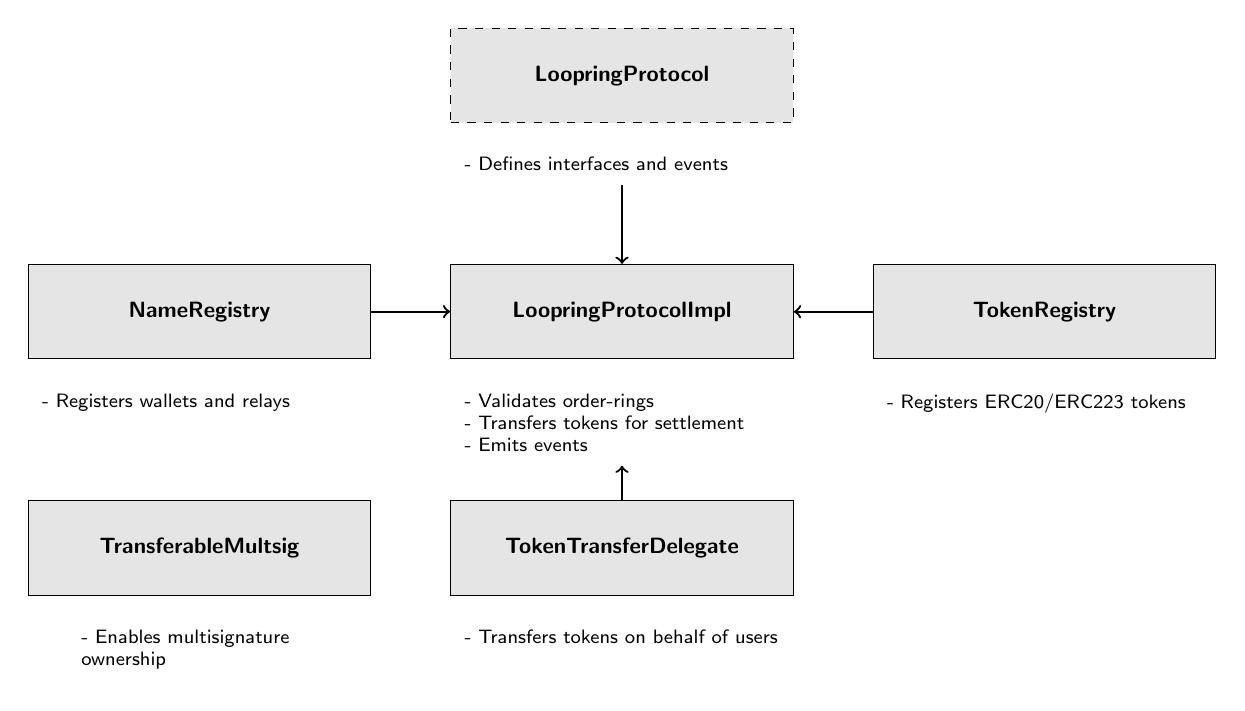
\begin{tikzpicture}
[node distance = 1cm, auto,font=\footnotesize,
% STYLES
every node/.style={node distance=3cm},
% The comment style is used to describe the characteristics of each force
comment/.style={rectangle, inner sep= 5pt, text width=4cm, node distance=0.25cm, font=\scriptsize\sffamily},
% The force style is used to draw the forces' name
force/.style={rectangle, draw, fill=black!10, inner sep=5pt, text width=4cm, text badly centered, minimum height=1.2cm, font=\bfseries\footnotesize\sffamily}] 

% Draw forces
\node [force] (impl) {LoopringProtocolImpl};
\node [force, dashed, above of=impl] (protocol_interface) {LoopringProtocol};
\node [force, left=1cm of impl] (nameregistry) {NameRegistry};
\node [force, right=1cm of impl] (tokenregistry) {TokenRegistry};
\node [force, below of=impl] (delegate) {TokenTransferDelegate};
\node [force, left=1cm of delegate] (multisig) {TransferableMultsig};

%%%%%%%%%%%%%%%
% Change data from here

% impl
\node [comment, below=0.25 of impl] (comment-impl) {- Validates order-rings\\
- Transfers tokens for settlement\\
- Emits events};

% nameregistry
\node [comment, below=0.25cm of nameregistry]{- Registers wallets and relays};

% protocol_interface
\node [comment, below=0.25 of protocol_interface](comment-interface) {- Defines interfaces and events};

% tokenregistry
\node [comment, below=0.25 of tokenregistry] {- Registers ERC20/ERC223 tokens};

% delegate
\node [comment, below=0.25 of delegate] {- Transfers tokens on behalf of users};

% PUBLIC POLICIES
\node [comment, text width=3cm, below=0.25 of multisig] {- Enables multisignature ownership};

%%%%%%%%%%%%%%%%

% Draw the links between forces
\path[->,thick] 
(comment-interface) edge (impl)
(nameregistry) edge (impl)
(tokenregistry) edge (impl)
(delegate) edge (comment-impl);

\end{tikzpicture}}
\caption{Smart Contracts}
\label{fig:smartcontracts}
\end{figure}
\end{center}

\subsection{Triển khai}
Các hợp đồng thông minh sau đây đã được triển khai trên mạng chính thức Ethereum:
\begin{small}
\begin{itemize}
\item LRC: 

\verb|0xEF68e7C694F40c8202821eDF525dE3782458639f|
\item TokenRegistry: 

 \verb|0xa21c1f2AE7f721aE77b1204A4f0811c642638da9|
\item TokenTransferDelegate: 

 \verb|0xc787aE8D6560FB77B82F42CED8eD39f94961e304|
\item NameRegistry:  

\verb|0x0f3Dce8560a6010DE119396af005552B7983b7e7|
\item LoopringProtocolImpl:  

\verb|0xc80BbAb86cED62CF795619A357581FaF0cB46511|
\item TransferableMultsig: 

 \verb|0x7421ad9C880eDF007a122f119AD12dEd5f7C123B|
\end{itemize}
\end{small}
\end{appendices}

\end{multicols}
\end{document}

